
% \documentclass[english]{ipsj}
%\documentclass[english,preprint]{ipsj}
\documentclass[english,preprint,JIP]{ipsj}

\usepackage{graphicx}
\usepackage{latexsym}
\usepackage{amsmath}
\usepackage[]{algorithm2e}

\def\Underline{\setbox0\hbox\bgroup\let\\\endUnderline}
\def\endUnderline{\vphantom{y}\egroup\smash{\underline{\box0}}\\}
\def\|{\verb|}


\setcounter{volume}{29}% vol25=2017
\setcounter{number}{1}%
\setcounter{page}{1}


\received{2021}{6}{1}
%\rereceived{2011}{10}{1}   % optional
%\rerereceived{2011}{10}{31} % optional
\accepted{2021}{6}{1}



\usepackage[varg]{txfonts}%%!!
\makeatletter%
\input{ot1txtt.fd}
\makeatother%

\begin{document}

\title{Startup Project B4}

\author{Elvin Mark Munoz Vega}{}[]

\begin{abstract}
    This is a summary report of the results obtained for the startup program
    assigned to the B4 students. First a quick review of what Nerual Networks
    are and their importance to the classification problems will be discussed as
    a review of some math concepts behind Neural Networks. Then, some of the
    more commonly used networks architectures will be implemented using the
    python framework for Deep Neural Networks: PyTorch. By using this framework,
    different network architectures are built and tested with different
    well-know image datasets : MNIST, KMNIST, CIFAR10, CIFAR100. The
    architectures discussed in this paper are: MLP (Multilayer Perceptron), CNN
    (Convolutional Neural Network), ResNet (Residual Network). Finally, based on
    these results, some analysis of the different implemented architectures is
    given.
\end{abstract}

\begin{keyword}
    PyTorch, Neural Networks, Convolutional Neural Network, ResNet.
\end{keyword}

\maketitle

%1
\section{Introduction}

Neural Networks has being proven as a very powerful tool within the Machine
Learning field. It can accomplish anything you would ever think. It can creates,
translates, geneartes, classify, etc. Specially when it comes to classify data,
it seems nerual networks are unbeatable. No matter what kind of data it is,
Neural Networks under the proper training and a proper data preprocessing will
be able to classify anything. Images, speech, text, actions, anything that can
be expressed as a sequence of numbers, can be classify with neural networks.
Neural Networks have come a long way since its creation in 1940's, since then it
has been evolving, adopting a more complex architecture so it can adapt to more
difficult classification task. In this paper some of the more famous and more
widely used networks will be discussed: MLP, CNN and ResNet.\\

Let's start first by describing what are neural networks. Well in a nutshell a
neural network is just a function that based on some parameters and some
specified operations it can transform an input into an output. In other words,
if $\vec{x}$ is my input then $\vec{y} = NN(W,\vec{x})$ would be my output. Here
$NN$ denotes a neural network. And that is basically it, depending on the types
of operations done inside the network and what kind of parameters you are using,
then you have a different architecture of a neural network but in the big
picture all looks like this simple function. Now, what we are looking for is a
the right parameters $W$ such that our network can predict or generate or
classify properly the data that we supply to it. In other words, if I have a
dataset $\mathbb{D} = \{\vec{x}_i,\vec{t}_i\}$, I want my model to exactly, or
approximately output $\vec{t}_i$ when I input $\vec{x}_i$ to it.

\begin{equation}
    NN(W,\vec{x}_i) = \vec{y}_i \simeq \vec{t}_i
\end{equation}

But how to do it? Well first we need to assign a number to a how close our model
is to the right output. So we can tell the neural network whether it is getting
close to the right output or not. This way to evaluates how accurate is the
neural network is called loss function.

\begin{equation}
    Loss = L(\vec{y}_i,\vec{t}_i)
\end{equation}

This function will have the property of being small or zero when $\vec{y}_i
    \simeq \vec{t}_i$ and have a huge value or a very high value when $\vec{y}_i$
gets "far" from $\vec{t}_i$.

Now our problem of finding the appropiate $W$ has become into a minimization
problem. Since finding the $W$ that makes the output of the neural network
$\vec{y}_i$ be close to $\vec{t}_i$, is similar to find the $W$ that make the
loss function minimum. And we have a very powerful tool in mathematics to
minimize functions that is called gradient descent.\\

As the method's name implies, the gradient descent methods uses the gradient of
the function you want to minimize to find the direction that it has to follow in
order to minimize the function.\\

\begin{equation}
    W_{k+1} = W_{k} - \alpha \frac{\partial L(\vec{y}_i,\vec{t}_i)}{\partial W}
\end{equation}

In this case we use a parameter $alpha$, that is known as learning rate, in
order to make the update more "smooth", less caothic and helps the model to
coverge quickly. It is important to notice that we use the negative of the
gradient since, that is the direction where the minimum point is. Think about a
parabola as an example, if you take the gradiend at some point around the
vertex, which is the minimum point, the gradient will always point outwards the
vertex. Therefore if we want to find the vertex we should go in the opposite
direction, thus the negative sign.\\

There are some problems of course with this method, to say the least. One of the
problems is that, the minimum that you are finding with this method, it is not
necessarily the global minimum, it can be just a local minimum. Another problem,
it is that you can fit perfectly your training data, the dataset $\mathbb{D}$
that we used to train our network, but that does not assure you that your
network will perform well with new data, this is called lack of generalization.
This are just some few problems from a larger list, but still this method has
been proven to be good enough to give some good results. There has been created
some methods that has helped to improve this method in order to avoid or to
somehow cope with the mentioned and unlisted problems, such as choose better
initial values, second order optimization and so on.\\

This is basically how neural networks work, kind of. New neural networks out
there may operate a little different but the main core is what it has been
explained until here. The basic process on how to train network goes a little bit like this:

\begin{algorithm}
    \KwData{$\mathbb{D} = \{\vec{x}_i,\vec{t}_i\}$}
    \KwResult{$W_{best}$}
    initialize $W_0$,$k=0$\;
    \While{$k<total epochs$}{
        \CommentSty{\textbf{Forward}}\;
        get the output of network using $W_k$\;
        $\vec{y}_i = NN(\vec{x}_i,W_k)$ \;
        calculate the loss \;
        $L = L(\vec{y}_i,\vec{t}_i)$ \;
        \CommentSty{\textbf{Backward}}\;
        calculate the gradiend \;
        $\frac{\partial L(\vec{y}_i,\vec{t}_i)}{\partial W}$\;
        \CommentSty{\textbf{Optimize}}\;
        update the parameters \;
        $W_{k+1} = W_{k} - \alpha \frac{\partial L(\vec{y}_i,\vec{t}_i)}{\partial W}$ \;
    }
    \caption{How to write algorithms}
\end{algorithm}

As it can be seen from the algorithm, the training process can be split into
three subprocess: Forwarding, Backwarding and Optimizing. The Forwarding is
pretty simple and straightforward, it just calculates the output from the neural
network using the current parameters. The Backwarding process calculates the
gradient by using basically chain rule among the layers within the neural
network. Since you are using chain rule you go from the more outward layer to
the first layer calculating the gradients, you are going backwards in this
process hence the name. Finally, in the Optimizing process, we used the
gradients we obtained in the previous step to update the parameters. This 3
subprocess repeats consecutively for a number of times or epochs.\\

%2
\section{Architectures}
%2.1
\subsection{MLP: Multilayer Perceptron}
This is one of the most simple networks that exists out there. The input data
$\vec{x}$ under some Linear Transformations, using some matrix $w$ and vector
$\vec{b}$, is transformed into an output $\vec{y} = w\vec{x} + \vec{b}$. Then
this output is transformed using an activation function, to give non-linearity
properties to this network. If no activation function is used at all, or just a
simple linear function, in other words $f(x) = x$ is used, then the
classification obtained but the network would not escape the linear domain,
making impossible to classify more complex distributed data. Hence non-linear
functions are used as activation functions such as: Sigmoid, Hyperbolic tangent,
ReLU, among others.\\

What it has been described until now, it is what a single layer does. This layer
is called Fully Connected Layer or FCC for short.

\begin{equation}
    \vec{o} = f(w\vec{x} + \vec{b})
\end{equation}

Here the matrix $w$ is called weights and the vector $\vec{b}$ is called bias.
In simple words, weights are how "strong" a neuron from the previous layer is
connected to a neuron in this layer. And the bias is a parameter that regulates
the threshold under which the neuron should "fire" or not to the next neuron.
And the activation function $f$ does exactly what the name suggests, a function
that tells the neuron how it should "fire", or how it should "activates". This
is of course just an analogy between this artificial neural networks and the
actual neural networks in our brains. If we see this from the math point of
view, it is just a linear transformation and a function evaluation for
non-linearity (similar to what kernel functions do).\\

Since we are dealing with a MULTI layer networks, that means that we are going
to stack multiple fully connected layers one after another. And the output of
one layer becomes the input of the next layer and so on until the last layer.

\begin{align*}
    \vec{o}_1 & = f(w_1\vec{x} + \vec{b}_1)       \\
    \vec{o}_2 & = f(w_2\vec{o}_1 + \vec{b}_2)     \\
    \vdots    &                                   \\
    \vec{o}_i & = f(w_i\vec{o}_{i-1} + \vec{b}_i) \\
    \vdots    &                                   \\
    \vec{o}_n & = f(w_n\vec{o}_{n-1} + \vec{b}_n)
\end{align*}

And that is basically the structure of this well know architecture. Now we just
have to train it by using some well known loss functions such as Mean Square
Error Loss or Cross Entropy Loss. Normally, for classification problems, the
Cross Entropy Loss are commonly used. And along with Cross Entropy Loss, it is
common practice, if not a must, to use a softmax layer at the end of the
network.\\

\subsection{Softmax Layer}
The softmax layers it is a statistical tool that allow us to transform our
output to a probability distribution. As we know, a probability distribution has
to fulfill an important property, that is the sum of all the probabilities
should be 1. The direct output of this fully connected layres does not
necessarily fulfill this, in fact they generally will not fulfill this. Another
property is that this values should be positive since they are probabilities,
and since we normally are using linear tranformations and activation functions
that can output negative values, therefore we need a transformation that fix
these 2 problems. This is done with the function describe in the following equation.
\begin{equation}
    y_{i} = \frac{e^{o_i}}{\sum_k e^{o_k}}
\end{equation}

This MLP network although efficient and useful suffers from some disadvantages.
One of these disadvantages is that it can is really heavy specially when we are
dealing with huge sized inputs. For example images. Images has a lot of
information, a really small image, such as the one used in the famous dataset
MNIST, has around 784 pixels (28x28). So if we were to use just one layer that
connects this 784 inputs to 100 neurons in the middle and then connect this
neurons to 10 output neurons (one ouput per each class) then we will have $78400
    + 1000 = 79400$ parameters in our weight matrices. Since each parameter is a
float number (8 bytes), our model will be around 0.6MB. This may seem a small
number but remember that we are using small images, just 28x28 images!. And as
we increase the resolution of the images to larger sizes our model will become
heavier and heavier quadratically. Also, as you may have already noticed, the
images are treated as a linear array in order to be processed in this network.
By flatten the image we are losing some import 2D information from it. Thus this
network will not be that good at classifying images. Here is where our next
network architecture came into play.

%2.2
\subsection{CNN: Convolutional Neural Network}

These networks were a game changer. Not just made our model less heavier but
also took advantage of the 2D structure of the information in images to improve
the accuracy of the model. The basic idea behind CNN is to extract some spatial
features from the image by applying filters. These filters are kind of the
weights used in the multilayer perceptron, but how we applied these filters to
the image are a quite different. Instead of doing some matrix multiplication, we
are going to use correlation. Which is basically a element wise multiplication
of submatrices within the image with the filters' elements and then adding them
all. We slide the filter around the image thus generating another image but with
different values. These new values represent some local characteristic of the
image. For example, if we use a filter that looks like a diagonal matrix, then
this filter will output high values when the submatrix within the image has a
diagonal line. Of course this is a very simple filter to examplify how filters
work. In reality, the filters that are found after training, find more complex
and abstract patterns that makes better image classification.

\begin{equation}
    y = I \star F + b
\end{equation}

Here $\star$ symbol represents the correlation operation. $F$ is the filter used
for the correlation and $b$ is the bias.\\

The correlation operation is defined as follow:\\
\begin{equation}
    [I \star F]_{ijk} = \sum_{pqr} I_{i+p,j+q,k+r}F_{pqr}
\end{equation}

When we perform backpropagation in the convolution layer we will use the
convolution operation (thus the name of convolution layer). Convolution
operation is defined as follows:

\begin{equation}
    [I * F]_{ijk} = \sum_{pqr} I_{i-p,j-q,k-r}F_{pqr}
\end{equation}

There other parameters that dictates how this operation is perform. Two of
those, and possible the main ones, are the padding and the striding. Padding is
basically how much margin, we should add to the image, by adding rows or columns
filled with zeros. The striding means how we should slide the filter around the
image, in other words how much the step should be.\\

What we have described so far is actually a kind of layer denominated
convolutional layer. Networks that uses this kind of layers are called
convolutional neural networks, but this does not mean that the network just uses
convolutional layers, it also includes activation function layers, fully
connected layers and other kind of layers that we will described now.

\subsection{MaxPool Layers and Average Layers}
These 2 layers are just ways to sub sample our input in order to reduce the size
of the input. From a sub matrix (or sub tensor) form the input we can just take
either the maximum value (MaxPool Layer) or the average value (Average Layer)
and by doing this for all the submatrices we can reduced the size of the input
matrix.\\

\begin{align}
    Y_{ijk} & = max(I_{ip:(i+1)p,jq:(j+1)q,kr:(k+1)r})  \\
    Y_{ijk} & = mean(I_{ip:(i+1)p,jq:(j+1)q,kr:(k+1)r})
\end{align}

\subsubsection{BatchNorm Layers}

\begin{align}
    \mu           & = \frac{\sum_{ijk} I_{ijk}}{N}                     \\
    \sigma^2      & = \frac{\sum_{ijk} (I_{ijk} - \mu)^2}{N}           \\
    \bar{x}_{ijk} & = \frac{I_{ijk} - \mu}{\sqrt{\sigma^2 + \epsilon}} \\
    Y_{ijk}       & = \gamma \bar{x}_{ijk} + \beta
\end{align}

\subsubsection{Dropout Layers}
This layer basically wants to avoid overfitting by "dropping" some values
randomly. By dropping we mean that we will change the actual value by zero
depending on a random choice. This makes the network to try to fit the train
data but never overfits because of the random factor.
\begin{align}
    Y_{ijk} = random(I_{ijk},0)
\end{align}

%2.3
\subsection{ResNet: Residual Network}
While trying to make more "deeper" networks, we encounter a problem and that is
the vanishing gradient. When we propagate the error from the output layer to
previous layer, the deeper we go, the smaller the gradient it becomes. Thus at
some point it will vanish completely or it will become so small that it will not
make it possible to properly update the parameters. This makes the network
accuracy to stop increasing or even decreasing while more layers are added. To
deal with this problem residual networks were introduced.\\

The main idea behind residual networks is to "shortuct" non contiguous layers so
layer $j-1^{th}$ is connected to layer $j+1^{th}$ skipping layer $j^{th}$. We
accomplish this shortcut by adding the input of layer $j-1^{th}$ to the output
of layer $j^{th}$, of course using some proper transformation to match the
dimension of this 2 tensors. The gradient makes use of this "shortcut" to avoid
being vanish and thus avoid the stated problem in the previous paragraph. This
block can be seen in Figure~\ref{fig:resblock}

\begin{figure}
    \centering
    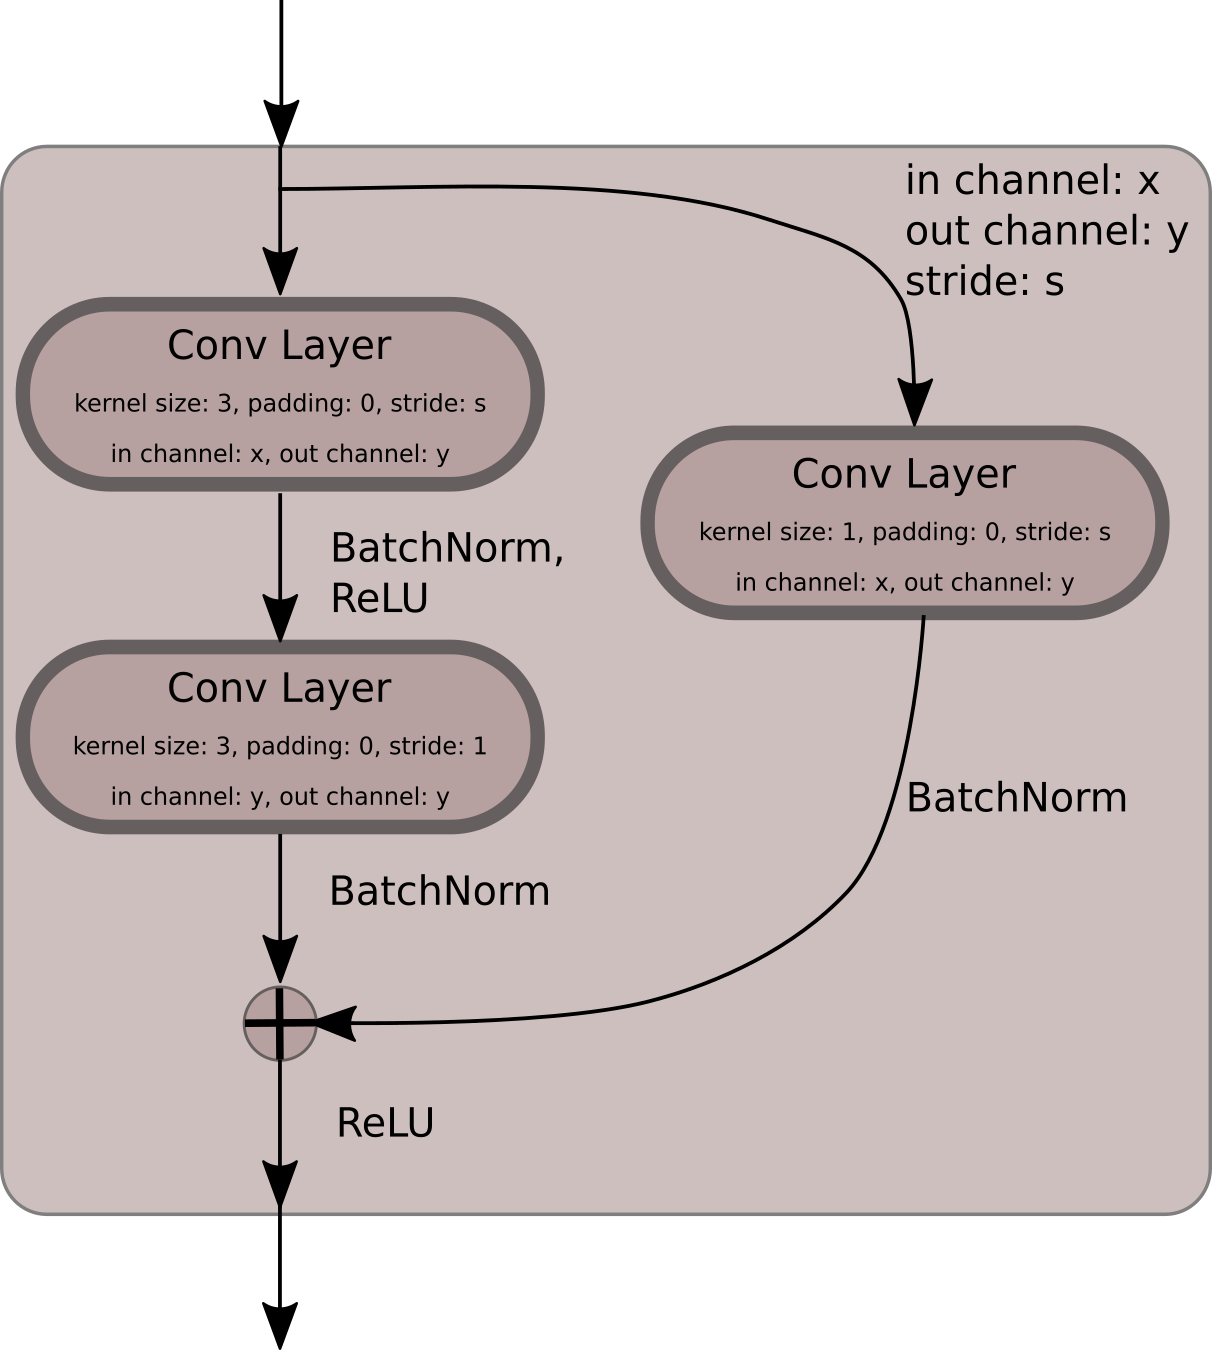
\includegraphics[width=0.5\textwidth]{img/resblock2.png}
    \caption{Residual Block}
    \label{fig:resblock}
\end{figure}
%3
\section{Results}
All of these explained architectures were implemented and tested with 4
well-known datasets: MNIST, KMNIST, CIFAR10, CIFAR100. The results are presented
in the following 4 sections with some brief observations.\\

\subsection{MNIST}
The MNIST is a famous dataset that contains images of hand written number digits
from 0 to 9. There are 60000 images in total, and the size of each image is of
28x28 which makes a total of 784 pixels per image. 50000 out of these 60000
images are used for training, while the others 10000 are used for validation.\\

For MNIST dataset we implemented 3 architectures: MLP, CNN (implemented by me)
and the famous LeNet \cite{lenet}. The Multilayer Perceptron architecture used
for this experiment consists by 2 layers which are detailed in
Figure~\ref{fig:mnist_mlp_arch} which consists simply of two layers. The first
one is a fully connected layer with 784 inputs and 300 outputs and then apply a
ReLU activation function. These 300 outputs are the inputs to the next fully
connected layer that has 10 outputs. These outputs correspond to the number of
clasess which in the case of MNIST is 10 corresponding to each digit.\\

\begin{figure}
    \centering
    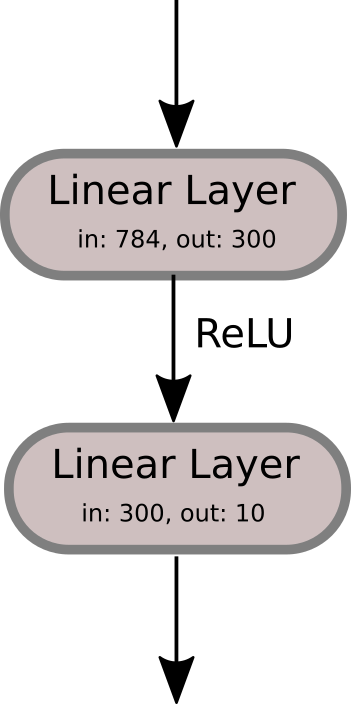
\includegraphics[width=0.2\textwidth]{img/mnist_mlp.png}
    \caption{MLP architecture for MNIST and KMNIST}
    \label{fig:mnist_mlp_arch}
\end{figure}

The CNN architecture used for this dataset is detailed in
Figure~\ref{fig:mnist_cnn_arch}. The first layer in this arcthitecture is a
convolutional layer with kernel size 3, padding and stride 1, and output 16
channels. After this layer we apply a ReLU activation function and a MaxPool
layer, with kernel size 2. We repeat these layers one more time, with the only
difference that the convolutional layer output 32 channels. These layers will
extract some spatial feature form the image, after we extracted these features,
we need to predict which digit the image is, based on these features. To do so,
we use some fully connected layers at the end.

\begin{figure}
    \centering
    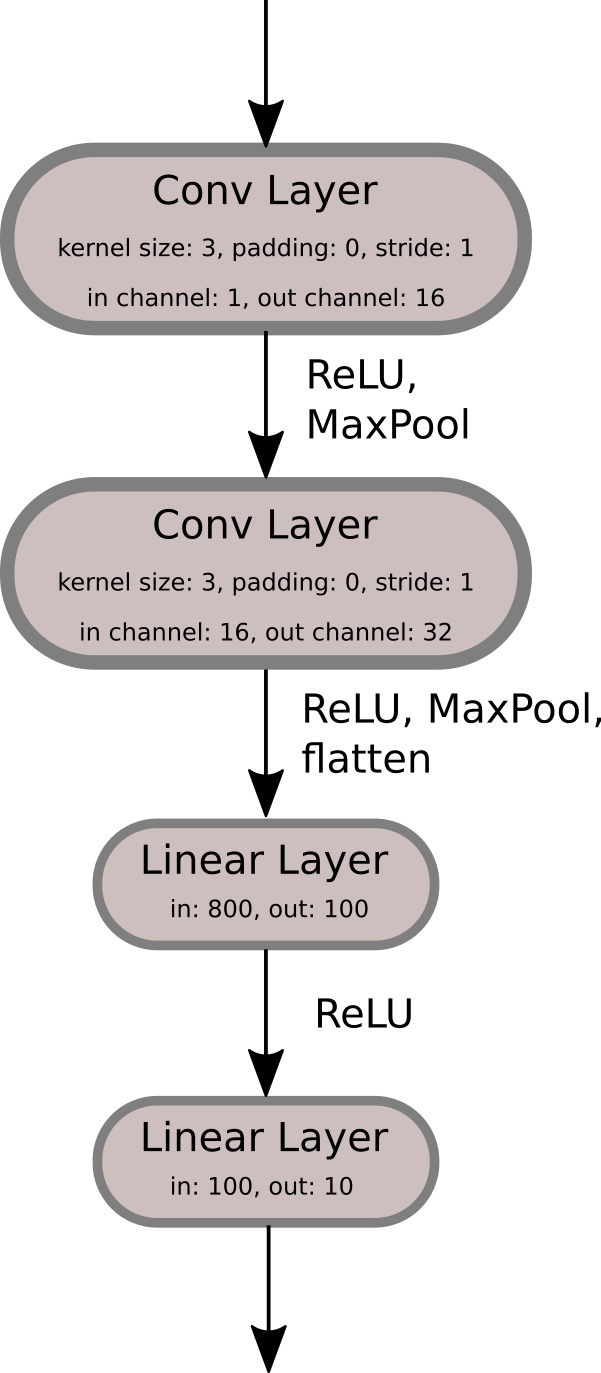
\includegraphics[width=0.3\textwidth]{img/mnist_cnn.png}
    \caption{CNN architecture for MNIST and KMNIST}
    \label{fig:mnist_cnn_arch}
\end{figure}

Also the famous LeNet network was implemented following the architecture
detailed in the original paper~\cite{lenet}.\\

All these architectures were trained using a constant learning rate of 0.01 and
for 50 epochs. Also the batch size taken for this training is of 500 images. The
results of this training for each architecture is shown in
Figure~\ref{fig:mnist_acc}. As we can see in the figure, the accuracy obtained
for all architectures are pretty much close, with the accuracy of the CNN being
the highest. In the case of MNIST dataset, the images, representing just
numbers, are pretty simple, there are not too much complex shapes in it. That is
why with a simple MLP we can obtain a pretty decent accuracy of $\sim 97.5\%$.
Of course a convolutional neural network will have a slightly better accuracy,
which in this case was $\sim 98.5\%$ for LeNet and $\sim 99\%$ for the
implemented CNN. The biggest difference among this architectures actually
appears in the memory size of the models. The MLP model weights approximately
1MB, while the CNN weights approximately 300KB.

\begin{figure}
    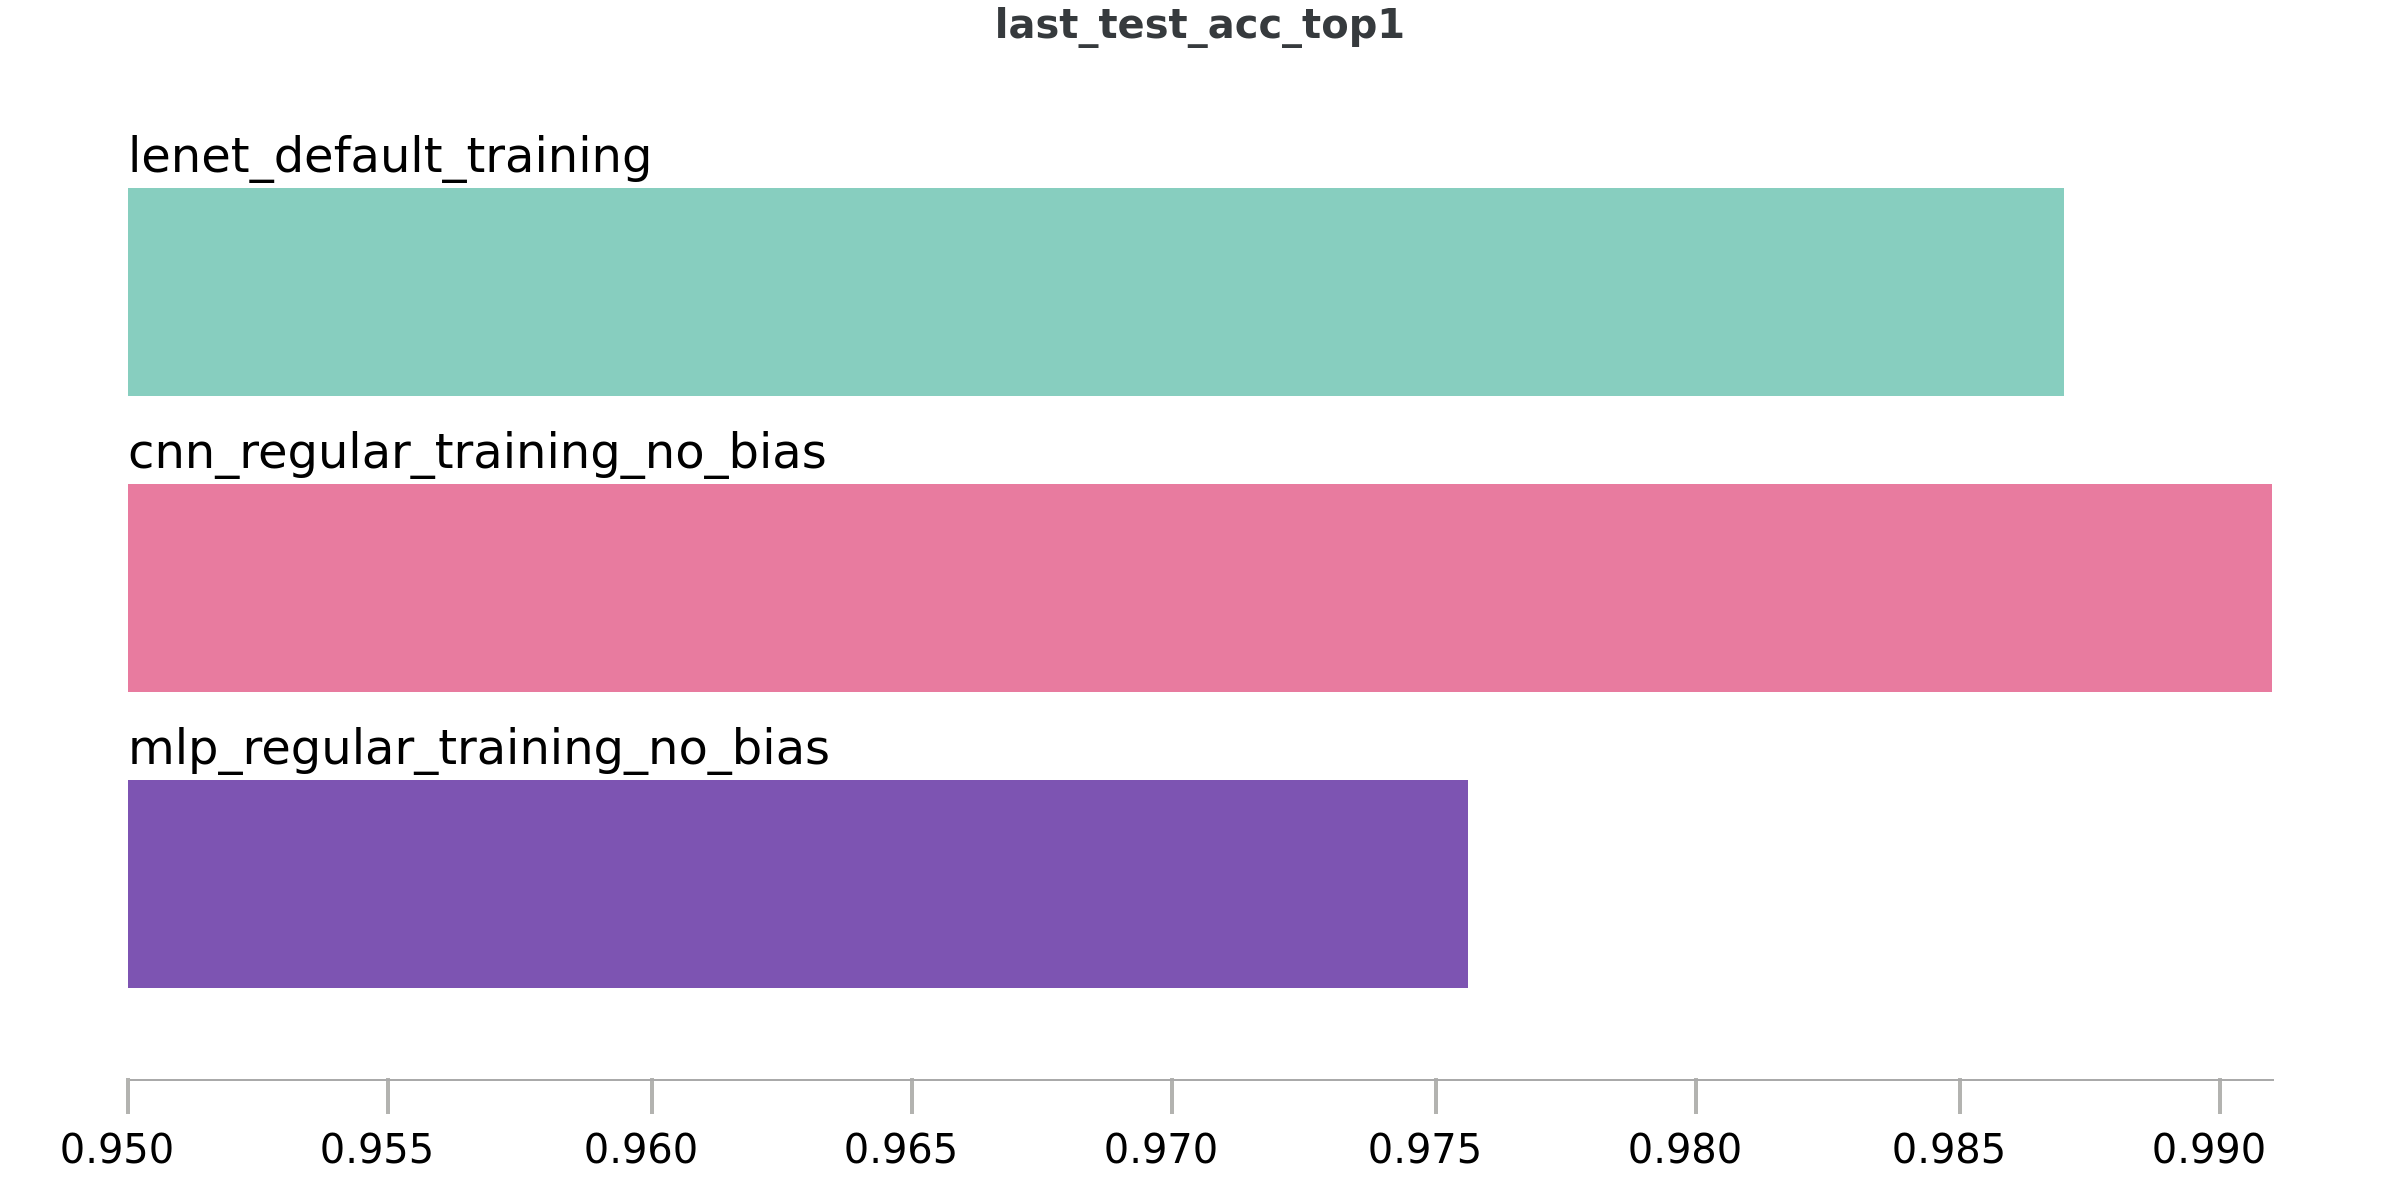
\includegraphics[width=0.5\textwidth]{img/mnist.png}
    \caption{Accuracy obtained for different architectures for the MNIST dataset}
    \label{fig:mnist_acc}
\end{figure}

\subsection{KMNIST}
Similarly with the MNIST dataset, the KMNIST dataset is also a dataset
containing images from 10 different classes. But this time instaed of having
hand written numbers, this dataset contains images of hand written hiragana
characters. The size of each image is the same as MNIST, 28x28. The number of
images in total as well as how many images are used for training and validation
are also the same with MNIST.\\

Since the datset is quite similar with MNIST, the same MLP and CNN architecture
as well as the LeNet architecture was used. During training the learning rate
was kept constant as in the previous case with MNIST dataset. In fact the same
learning rate was used, 0.01. Also the number of epochs was 50, and the batch
size was also of 500 images.\\

The results for the trained architectures are shown in
Figure~\ref{fig:kmnist_acc}. As it can be seen from the figure, in this case
even though the obtained accuracies were quite decent, above $90\%$, the
accuracy between architectures were quite more noticeable. This time the MLP
network did not perform as well as before, given an accuracy of $\sim 90.5\%$.
The LeNet network came a little bit better with an accuracy of $\sim 93.5\%$ and
the CNN network came first with an accuracy of $\sim 95\%$. In this case, the
hiragana characters showed a little bit more complex shapes than the numbers and
thus a simple MLP cannot tell them apart as well as a convolutional network.\\

\begin{figure}
    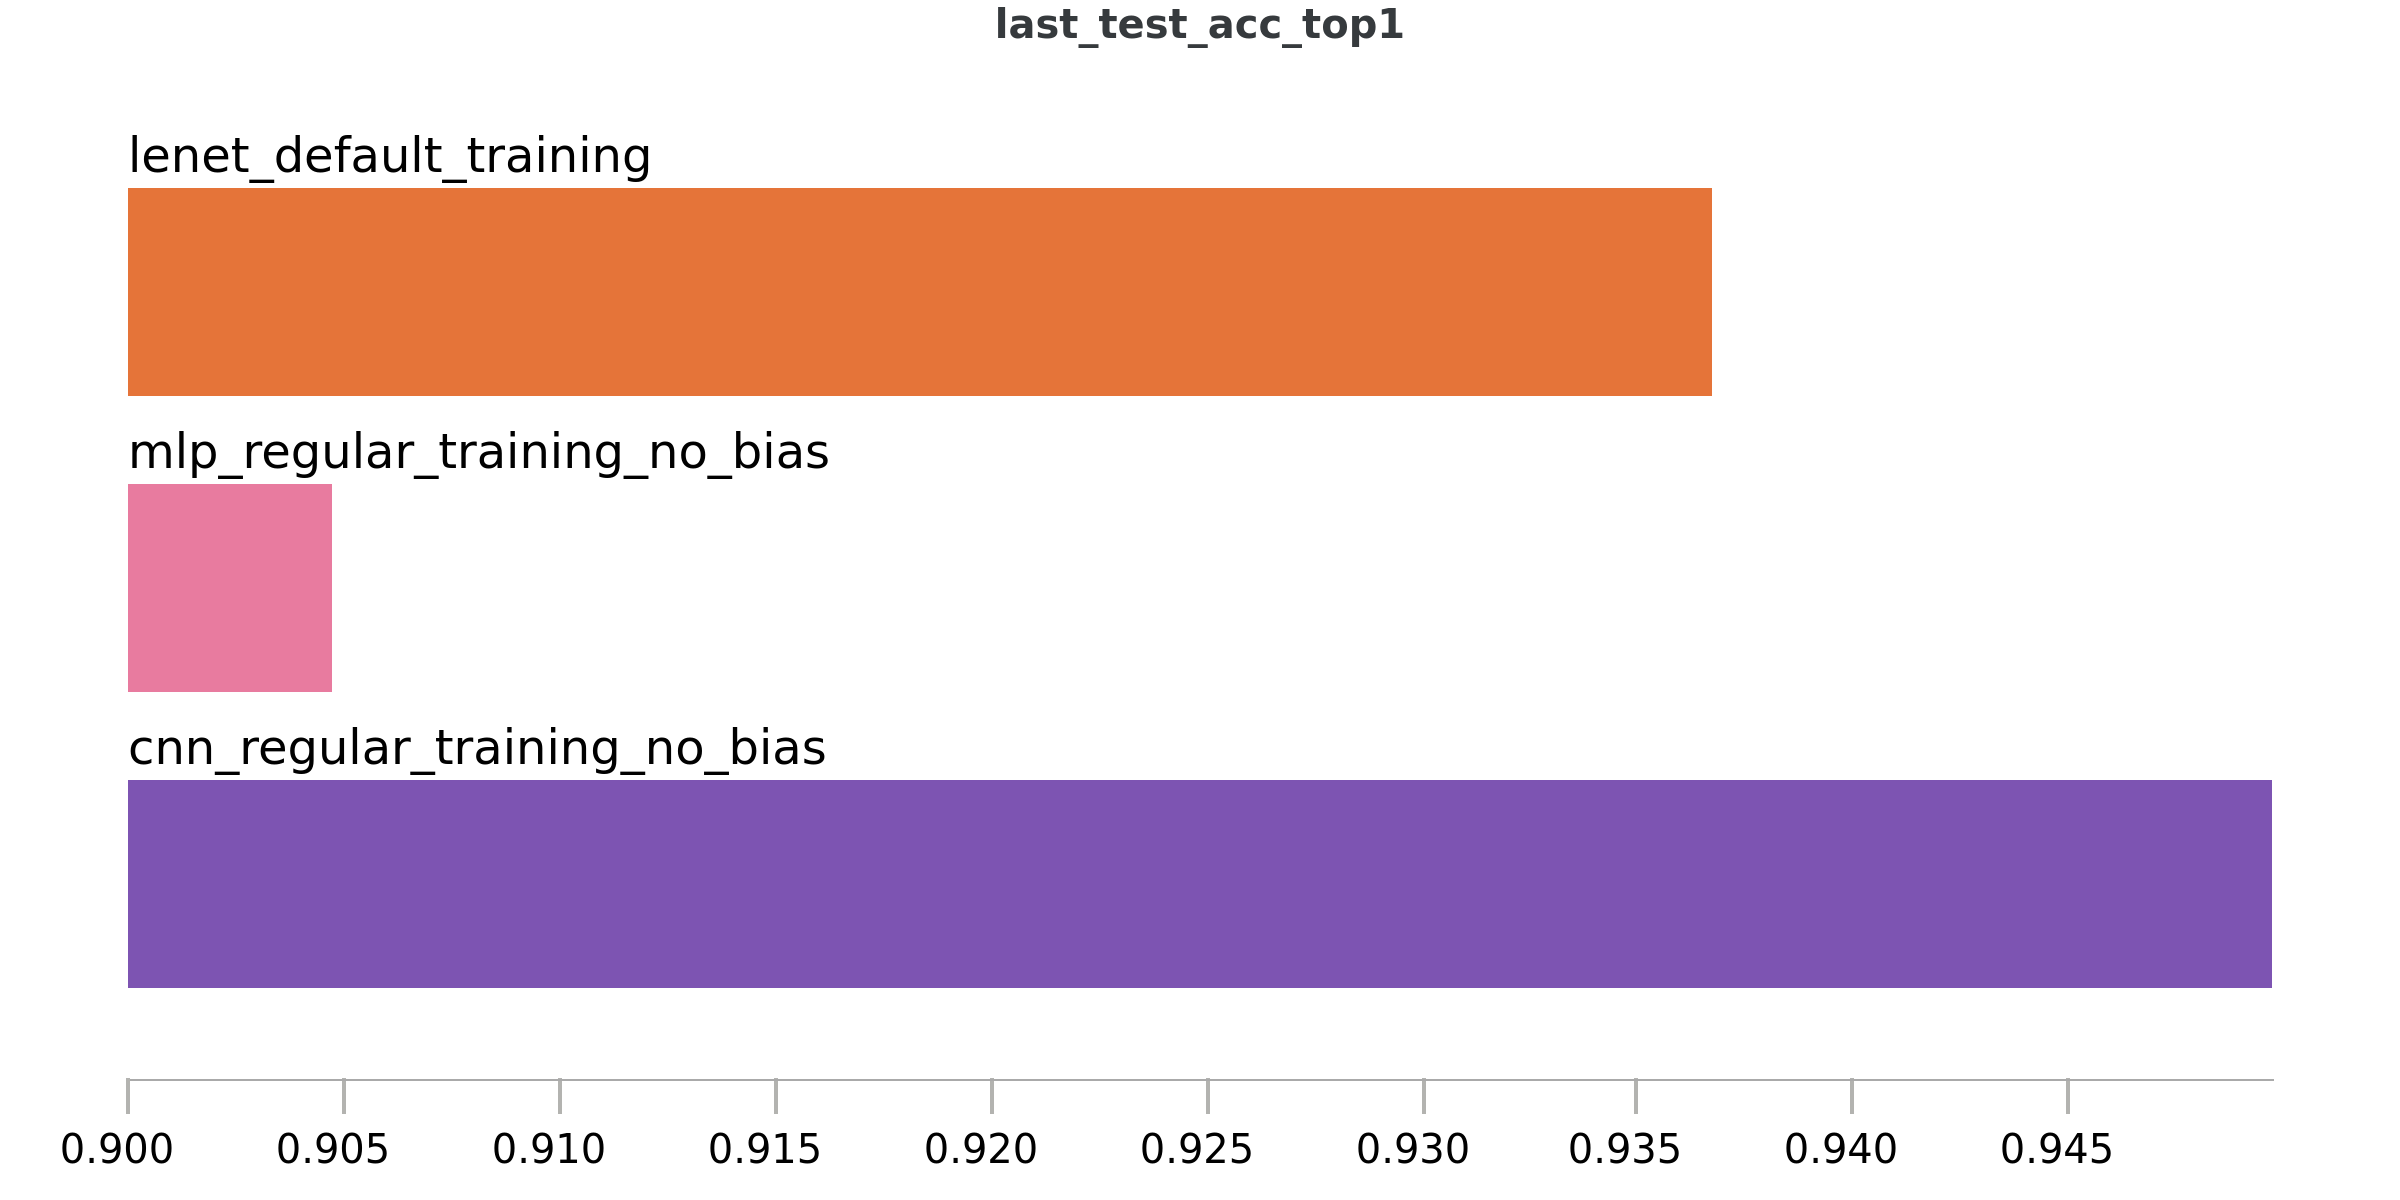
\includegraphics[width=0.5\textwidth]{img/kmnist.png}
    \caption{Accuracy obtained for different architectures for the KMNIST dataset}
    \label{fig:kmnist_acc}
\end{figure}

\subsection{CIFAR10}
The CIFAR10 is another famous dataset used a little bit more often than MNIST
nowadays. This dataset consists of images again from 10 different classes. But
this time this images are not simple numbers or characters or even black and
white images as the previous mentioned datasets, but instead they are colored
images of more real things that we can see every single day such cars, trucks,
airplanes, etc. The size of each image is also differente, 32x32. The total
number of images is similar to previous mentioned datasets, 60000. The
distribution among training and validation images is also the same.\\

The MLP architecture used this time has 3 layers. The first fully connected
layer takes an input of $3\times 32 \times 32 = 3072$ numbers and outputs $256$
numbers. Then a ReLU activation function is used. The next fully connected layer
takes those $256$ and outputs $32$ numbers. After this operation a ReLU
activation function is used. The last layer takes these $32$ numbers and output
$10$ numbers that represents the probability of the image to belong to each
class.\\

\begin{figure}
    \centering
    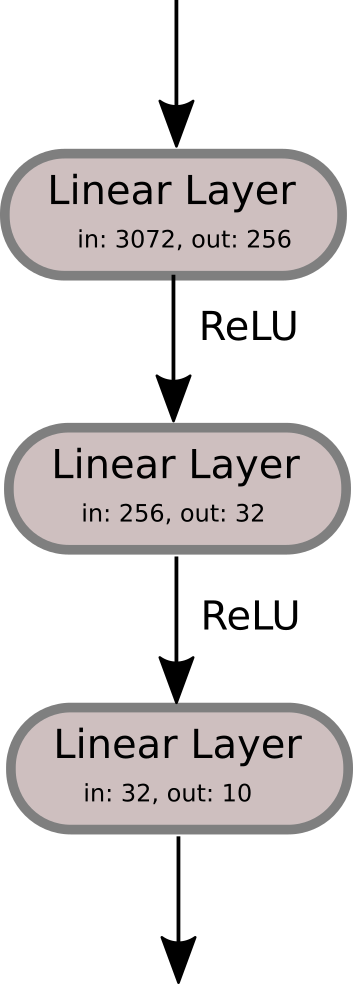
\includegraphics[width=0.2\textwidth]{img/cifar_mlp.png}
    \caption{MLP architecture used for CIFAR10}
    \label{fig:cifar_mlp}
\end{figure}

The CNN architecture used for this dataset is shown in
Figure~\ref{fig:cifar_cnn}. As it can bee seen from the image, this time 3
convolutional layers were used. In between this conovlutional layers there are
BatchNorm, ReLU activation functions and MaxPool Layers. At the end of this
sequence of convolutional layers, there are 2 fully connected layers that are
the ones that will do the classification based on the extracted features from
the convolutional layers.\\

\begin{figure}
    \centering
    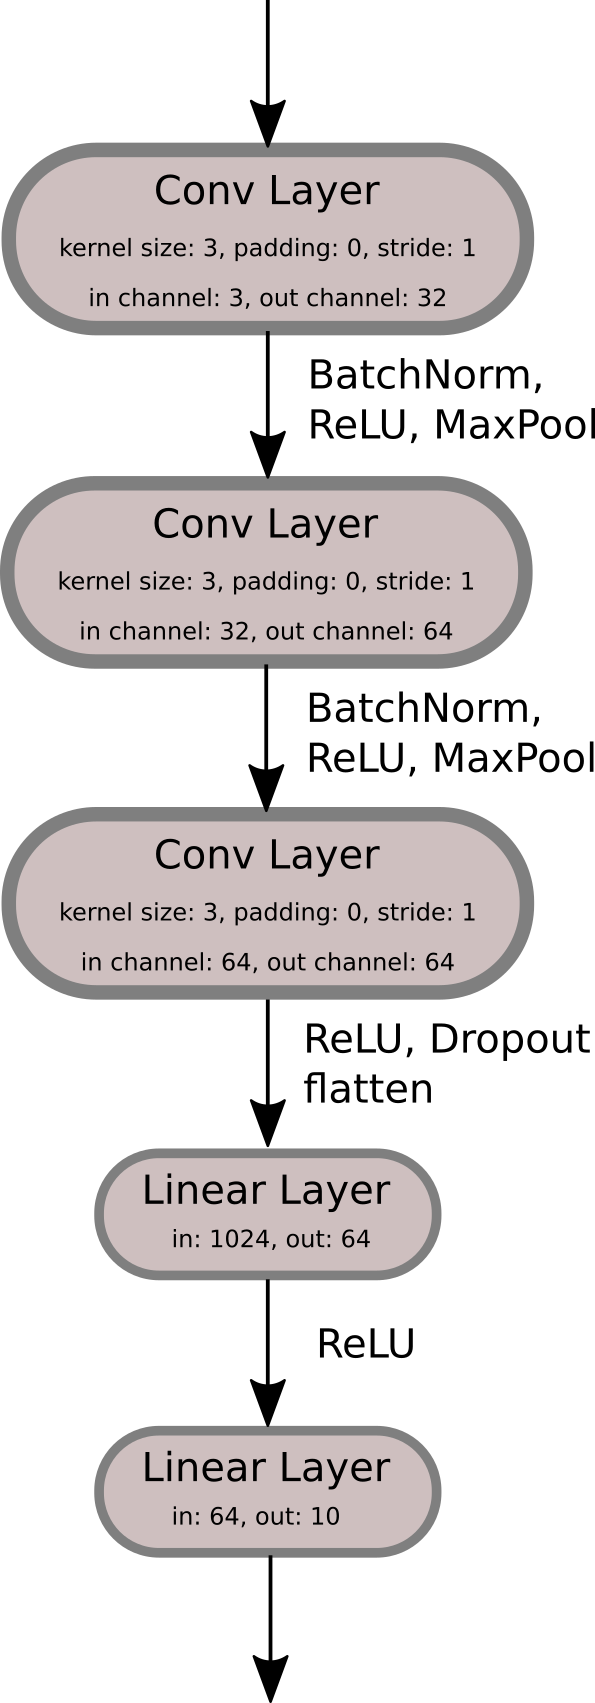
\includegraphics[width=0.3\textwidth]{img/cifar_cnn.png}
    \caption{CNN architecture used for CIFAR10}
    \label{fig:cifar_cnn}
\end{figure}

As a reference, the convolutional neural network AlexNet~\cite{alexnet} was also
implemented. This network was implemented for the ImageNet dataset, which deals
with larger images, so some adjustmens to the first layers had to be made as
well as the last layers, since we just have 10 classes and not 22000 classes as
the ImageNet dataset has.\\

Using the concepts of ResNet layers introduced in the previous section, 2 ResNet
Networks were implemented. The first resnet network architecture can be seen in
~\ref{fig:cifar_resnet} and for comparison the resnet network detailed in
~\cite{resnet} was also implemented. This architecture can be seen in
Figure~\ref{fig:cifar_original_resnet}. As it can be seen both arcthitectures
are quite similar with one of the main difference being the number of output
channels.\\

\begin{figure}
    \centering
    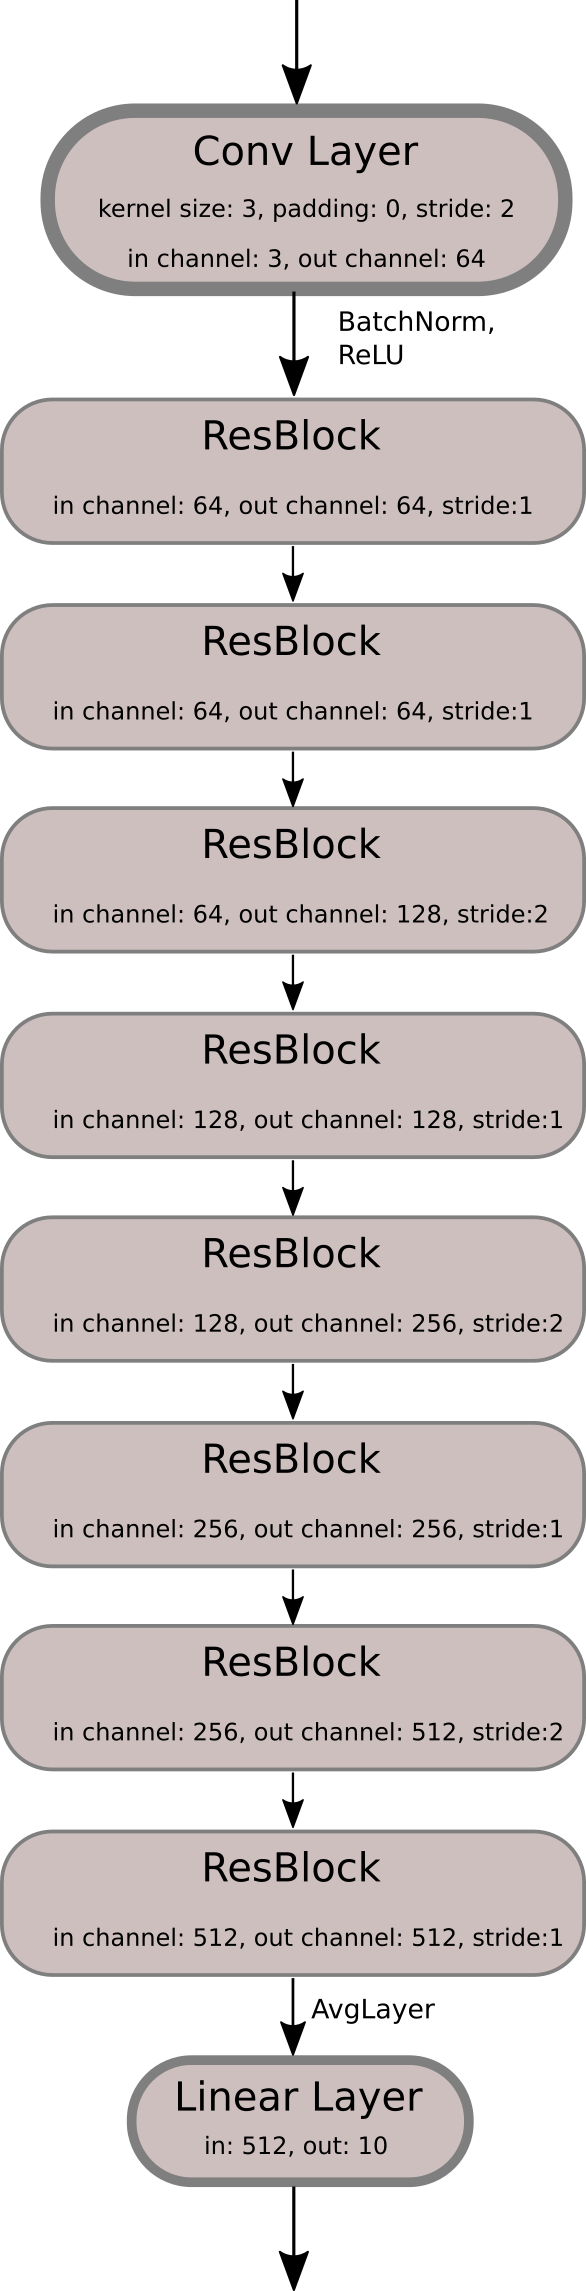
\includegraphics[width=0.3\textwidth]{img/cifar_resnet.png}
    \caption{ResNet architecture used for CIFAR10}
    \label{fig:cifar_resnet}
\end{figure}

\begin{figure}
    \centering
    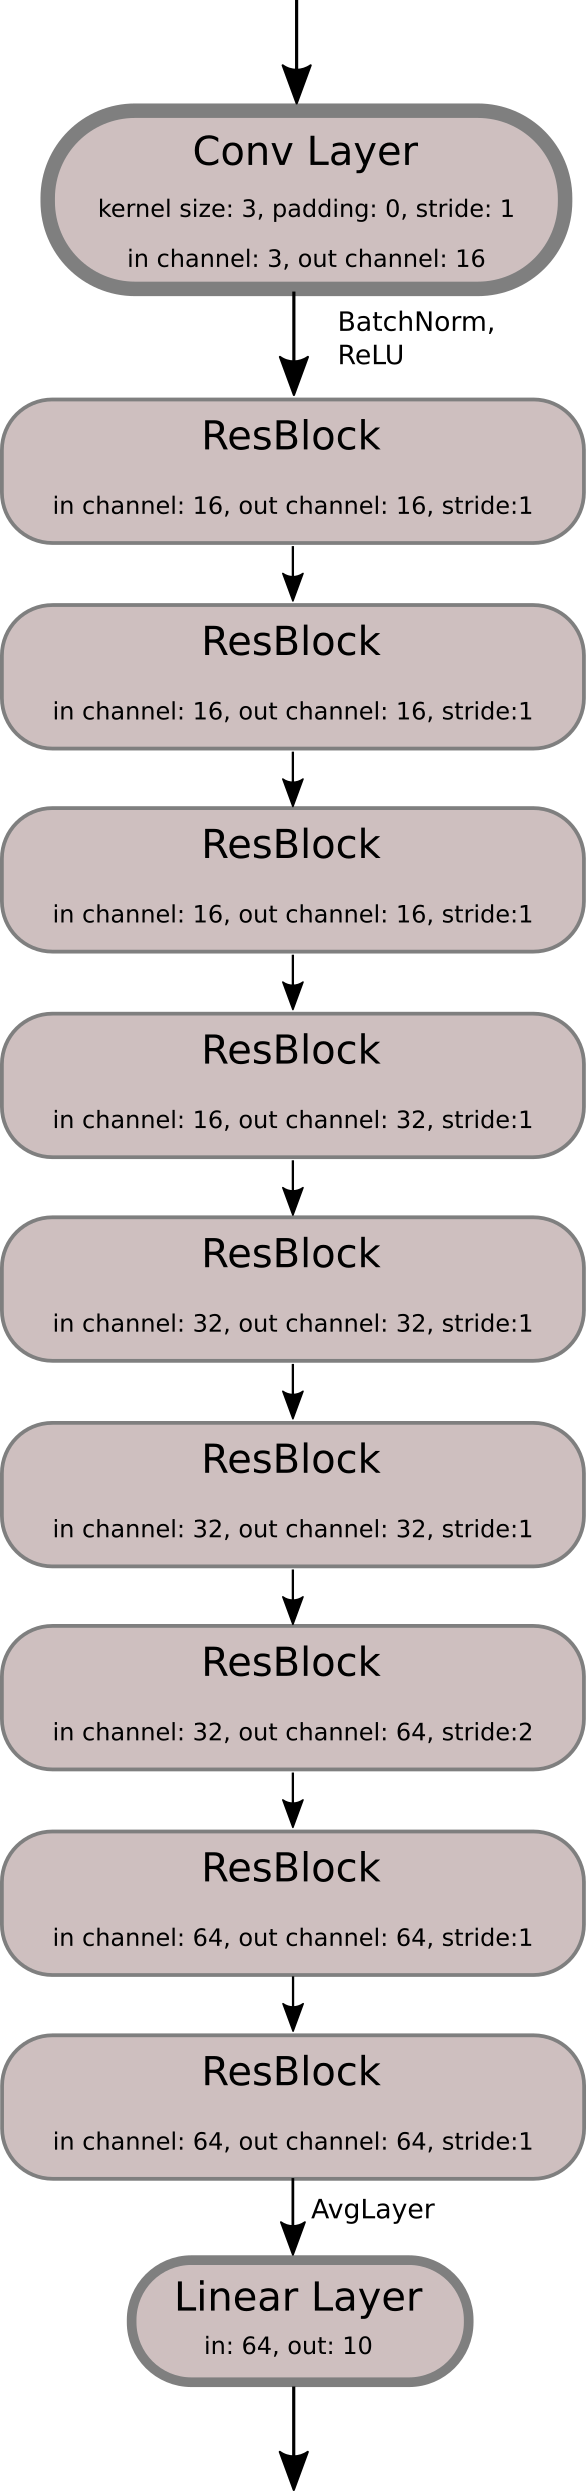
\includegraphics[width=0.3\textwidth]{img/cifar_resnet2.png}
    \caption{Original ResNet~\cite{} architecture used for CIFAR10}
    \label{fig:cifar_original_resnet}
\end{figure}


For the training process we use the step learning rate scheduler specified in
Table~\ref{tab:learning_rate}. Also we applied some data augmentation to the
dataset. The dataset augmentation is a technique used during training that
allows better generalization of the model, in other words make the model perform
better under new images thus improving its accuracy. Some of the more common
data augmentation are Image Flip, Image Rotation, Image blurr, Image Crop, etc.
In this case, Image Flip, Image Rotation and Image Crop were applied randomly to
the image during training. This randomness helps with the overfitting problem
while also improving generalization of the model.\\

\begin{table}
    \centering
    \caption{Learning Rate Scheduler used for models' training using CIFAR10 and CIFAR100 dataset}
    \begin{tabular}{c c}
        Epoch range & Leraning Rate \\
        \hline                      \\
        0 ~ 14      & 0.1           \\
        14 ~ 29     & 0.02          \\
        29 ~ 39     & 0.004         \\
        39 ~ 49     & 0.0008
    \end{tabular}
    \label{tab:learning_rate}
\end{table}

The results of the training for all of these architectures are shown in
Figure~\ref{fig:cifar10_acc}. As it can be seen from the figure, this time the
MLP network perform not as good as it did previously. It just reached an
accuracy of about $40\%$. This was expected since now we are dealing with more
colored complex images, so a simple fully connected layer will not perform as
well as a convolutional layer. Of course, if we increase the number of neurons
in each layer we may be able to increase the accuracy of the network but the
models size, in other words, the number of parameters will become ridiculously
large making the model very heavy unnecessarily. Also this model with millions
of parameters will likely to overfit and have a poor generalization for new
images.\\

As expected the accuracy for convolutional networks were much higher than the
MLP's accuracy. The CNN implemented for this experiment as well as the AlexNet
performed quite good obtaining an accuracy in the range of $75\% \sim 80\%$.
Even though this is almost as twice as the accuracy obtained from an MLP
network, it is still not good enough. Unfortunately if we just keep adding
layers, the accuracy will not improve but it will decrease due to vanishing
gradien problem. And here is were ResNets came to play.\\

For the ResNets implemented for this experiment, it was found a noticeable
improvement in the accuracy. The ResNet that it was proposed in the original
paper~\cite{resnet} obtained an accuracy of about $89\%$ and the ResNet
implemented that I implemented for this experiment obtained an accuracy of about
$91\%$. The accuracy difference is not that much but the models' weights are
very much different. Sine my ResNet model used a lot more parameters, it weights
around 40MB while the ResNet proposed in \cite{resnet} weights just around 1MB.\\

\begin{figure}
    \centering
    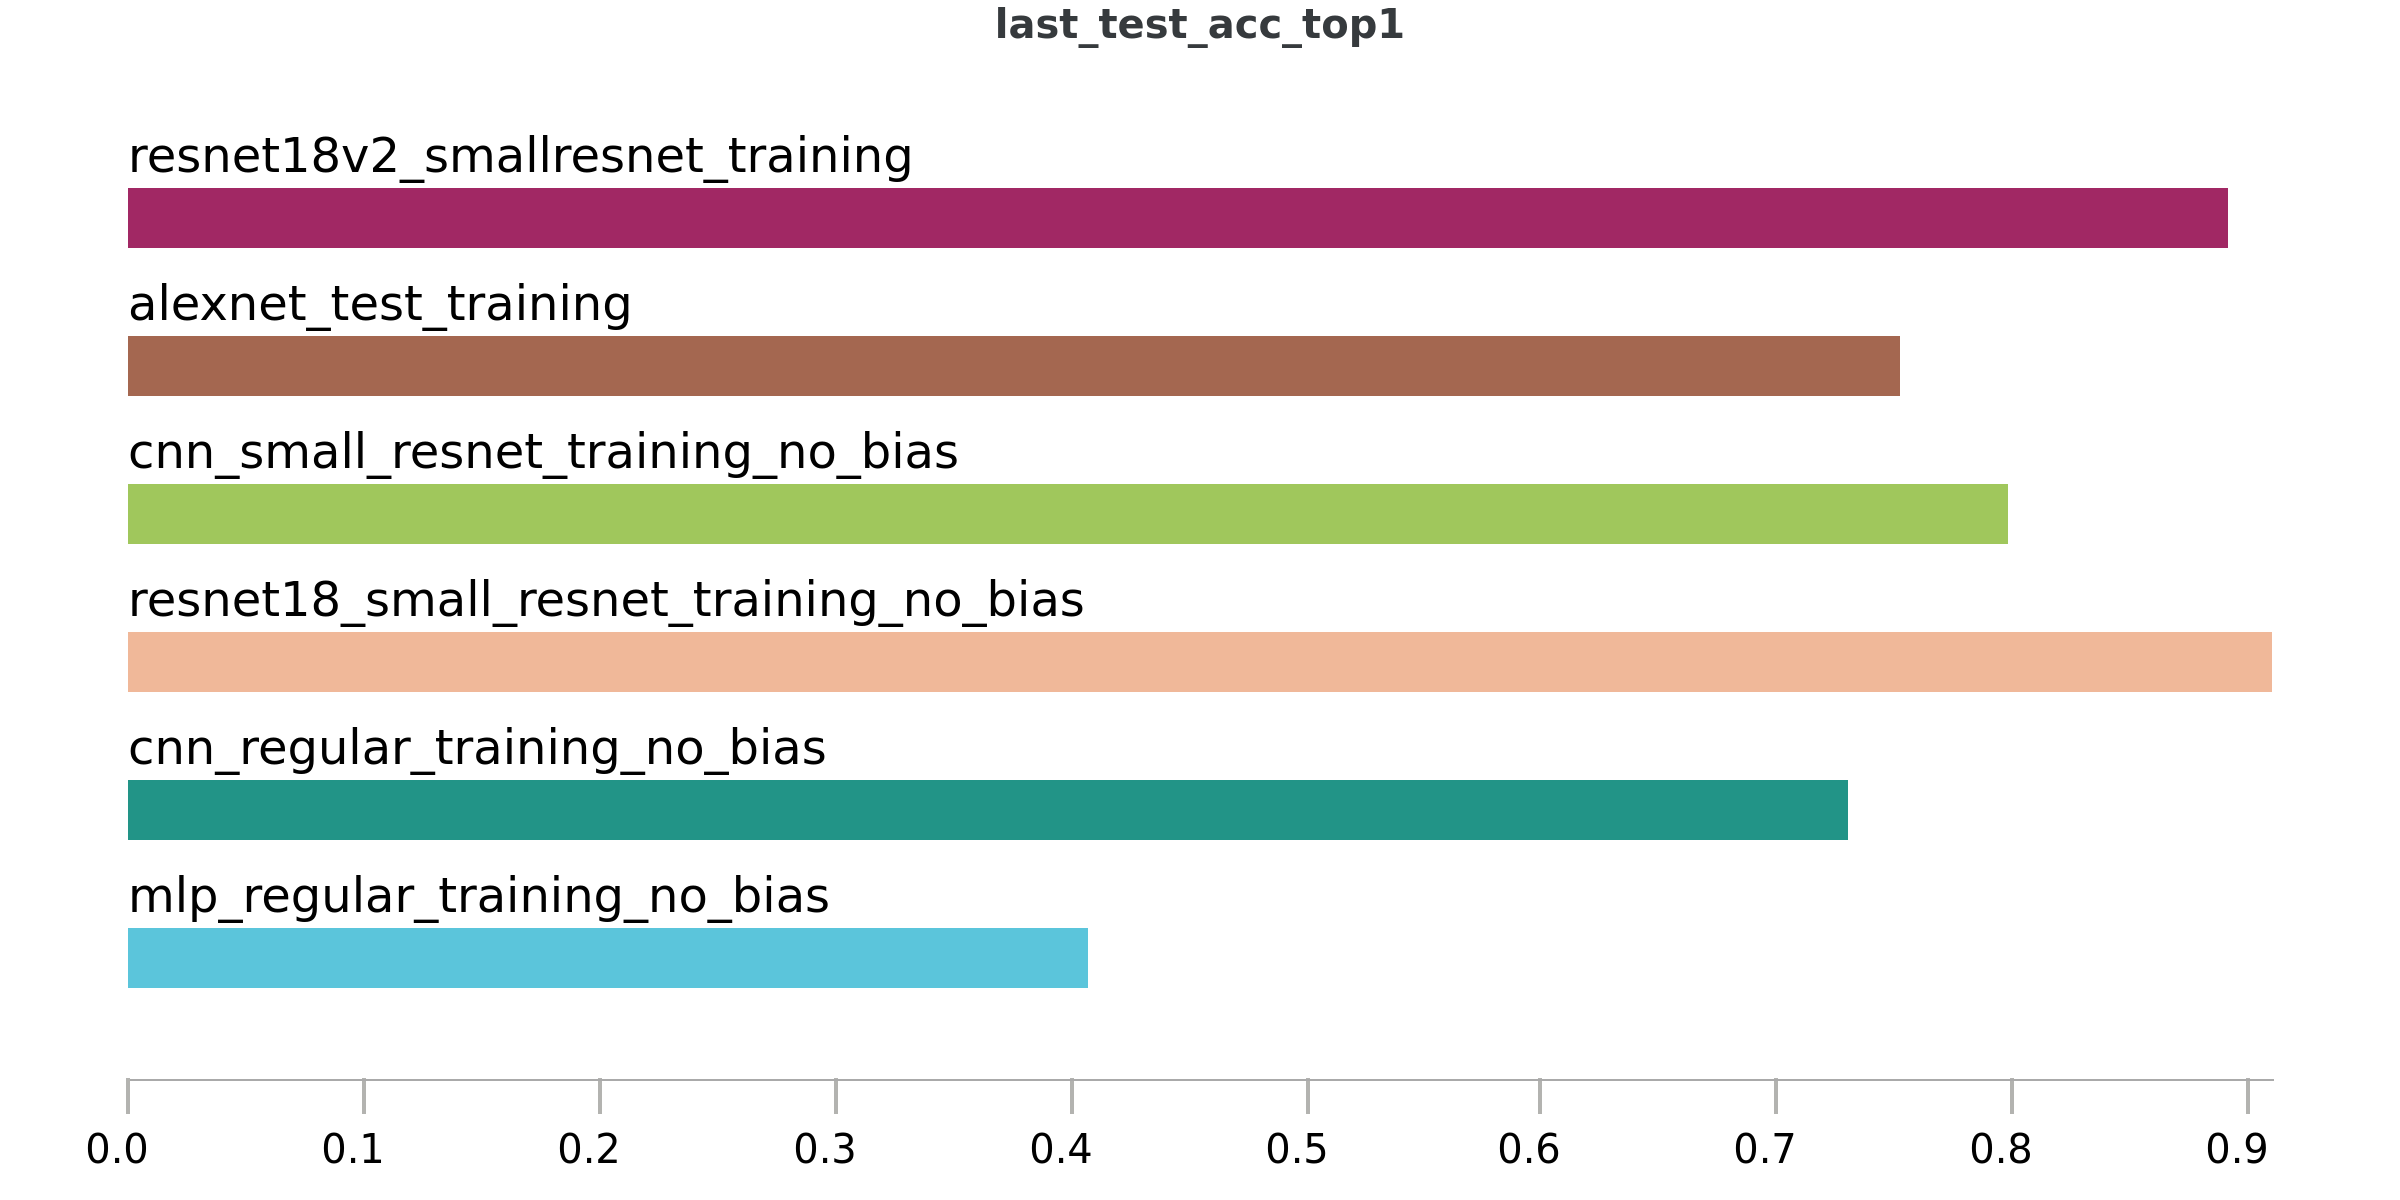
\includegraphics[width=0.5\textwidth]{img/cifar10.png}
    \caption{Accuracy obtained for different architectures for the CIFAR10 dataset}
    \label{fig:cifar10_acc}
\end{figure}

\subsection{CIFAR100}
The last dataset used during this startup program was the CIFAR100. This dataset
is similar to CIFAR10 but instead of just having 10 classes of images, it has
100 classes. But it has the same amount of images, 60000 images. And each image
is of the same size as before, 32x32. Also the number of images used for
training and validation is the same as in CIFAR10.\\

Since the image dimension are the same with CIFAR10, the same architectures were
used for this dataset. With the only difference being the last layer, the last
fully connected layer that performs the classification using the features
extracted in previous layers. In this last layer, the number of output neuron
were changed from 10 to 100.\\

The training process were the same as the one used with CIFAR10. The same
learinig rate scheduler (Table~\ref{tab:learning_rate}) was used. The same data
augmentation technique was used.\\

The accuracy obtained for this models are shown in
Figure~\ref{fig:cifar100_acc}. As it can be seen, a trend similar to the one
found in CIFAR10 was obtained. The MLP accuracy was the lowest, this time it
just reached $15\%$ accuracy. The simple convolutional networks, including the
AlexNet, also did not obtained aceptables accuracy, around $40\% \sim 50\%$. The
one with the highest accuracy is again the ResNet, obtaining an accuracy of
around $70\%$.\\

\begin{figure}
    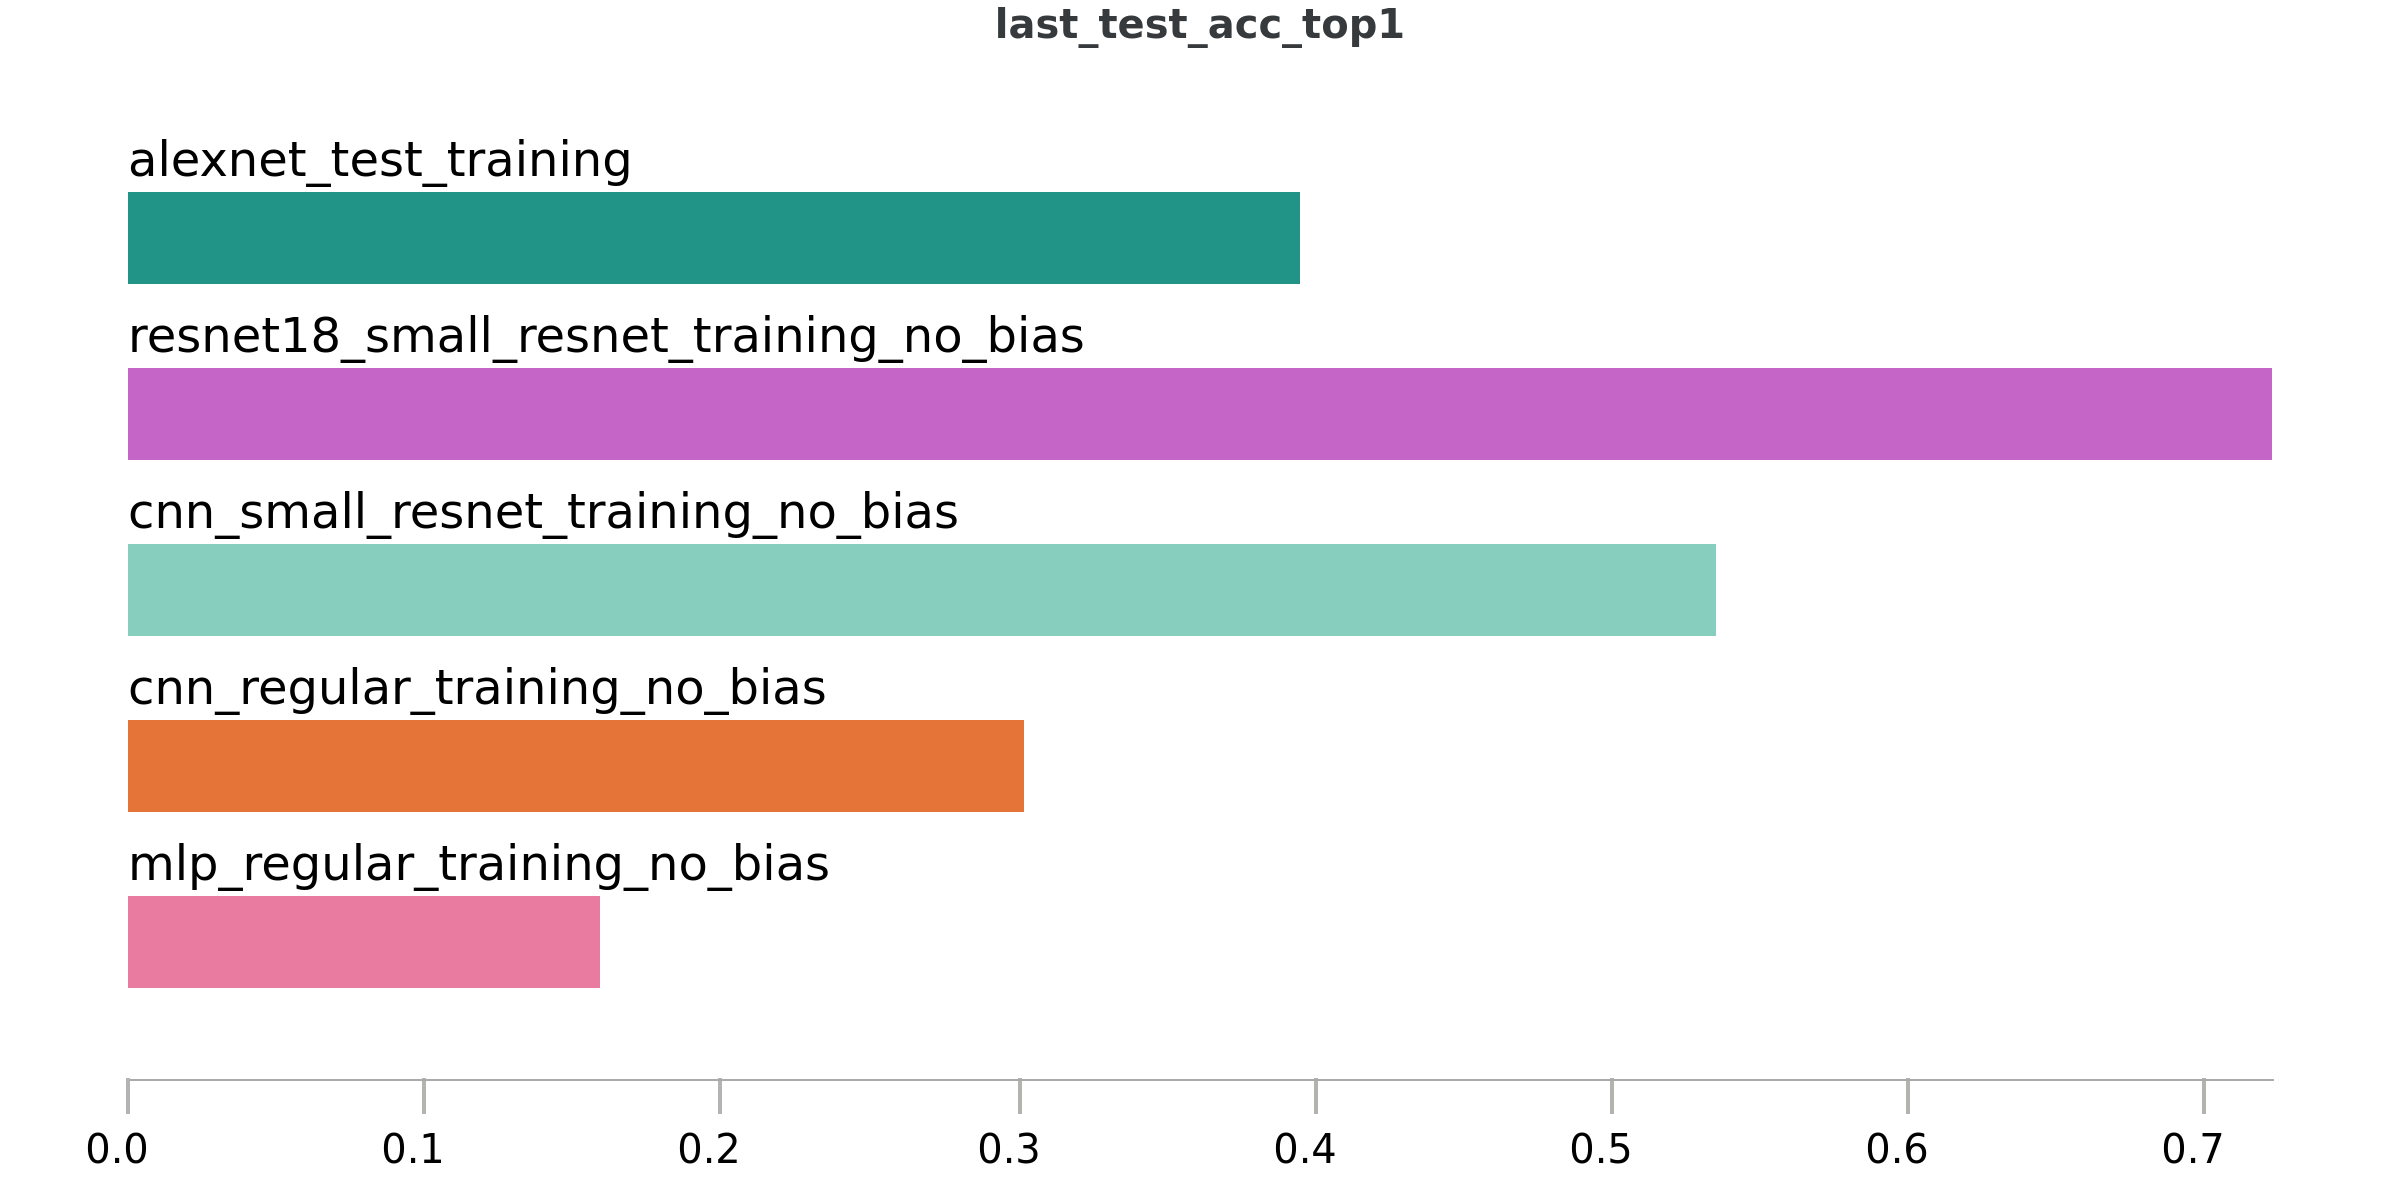
\includegraphics[width=0.5\textwidth]{img/cifar100.png}
    \caption{Accuracy obtained for different architectures for the CIFAR100 dataset}
    \label{fig:cifar100_acc}
\end{figure}

%4
\section{Discussion}
From the results of the experiments, it is clear that conovlutional networks are
much powerful than simple fully connected layers. They allow the neural networks
to recongize more complex and abstract shapes from the images without making the
model too heavy. By combining the power of neural networks and the idea behind
residual networks, we can make deeper networks that allow us to accomplish more
complex classification and recognition taks. There is not doubt that
convolutional layers made a huge impact to the computer vision world since they
were first introduced around 1998. \\

From the experiments we can also noticed some important characterisitc about the
usage of some layers. For example, we were able to notice that when using
BatchNorm Layers, we should not use Dropout Layers, since the combination of
these two layers affects the accuracy of the network. Also it was seen that we
should not use bias in the Convolutional Layers when we are using a BatchNorm
Layer after the Convolutional layer. Since the BatchNorm Layer will get rid of
the bias values at the moment of rescaling using the mean as the center.\\

Even though MNIST has already become a way too simple dataset and nowadays it
cannot be used for benchmarking, instead ImageNet or more complex datasets are
often used, we can still learn a lot by experimenting with it. For example, we
can see how the filters of the convolutional networs look like after training,
as it can be seen in Figure~\ref{fig:cnn_filters}. Allowing us to understand
what kind of features the network is trying to extract from the image.\\

\begin{figure}
    \centering
    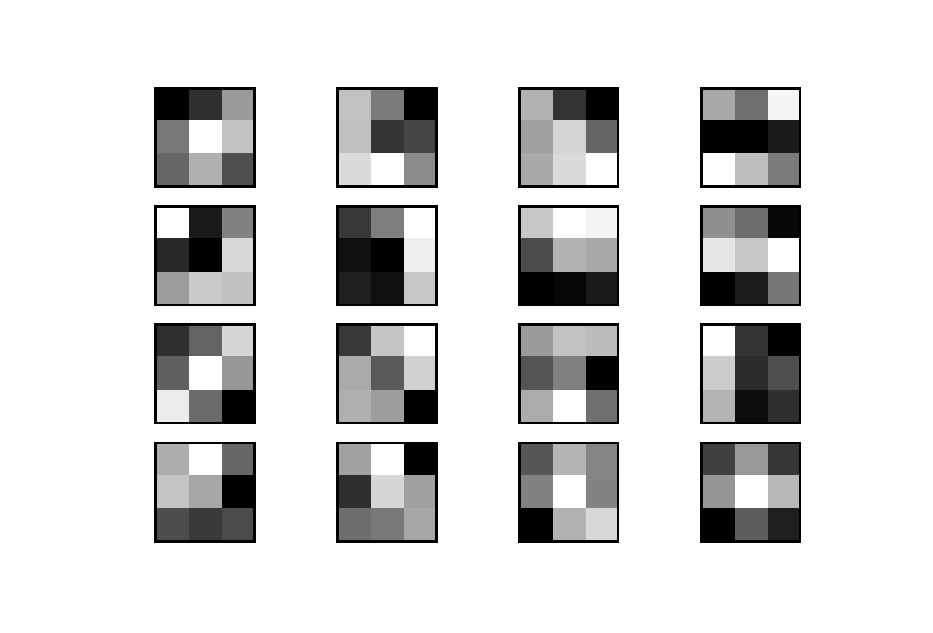
\includegraphics[width=0.5\textwidth]{img/mnist_cnn_filters_first_layer.eps}
    \caption{Filters of the first layer of the trained CNN for MNIST}
    \label{fig:cnn_filters}
\end{figure}

%5
\section{Conclusion}
By implementing these different architectures and applying them to the
classification fo different datasets using different ways of training, we can
get a deep understanding of the basics of Deep Nerual Networks.

\begin{thebibliography}{99}
    \bibitem{zerodl}%1
    Koki, S. :
    Deep Learning from scratch,
    O'Reilly, Inc,
    Japan (2016).

    \bibitem{dltorch}%2
    Stevens, E., Antiga, L. and Viehman, T.:
    Deep Learning with PyTorch,
    Manning, Shelter Island (2020).


    \bibitem{lenet}%3
    LeCunn, Y., Bottou L., Bengio Y., Haffner P.:
    Gradiend-Based Learning Applied to Document Recognition
    IEEE (1998)

    \bibitem{alexnet}
    Krizhevsky, I. Sutskever, and G. E. Hinton,
    ImageNet Classification with Deep Convolutional Neural Networks
    Advances in Neural Information Processing Systems 25 (2012)

    \bibitem{resnet}%2
    Kaiming, H., Xiangyu, Z., Shaoqing, R. and Jian, S.:
    Deep Residual Learning for Image Recognition,
    {\it CoRR},
    abs/1512.03385,
    (2015)
\end{thebibliography}

\end{document}
